\section{eo\-Uniform\-Gene\-Chooser$<$ EOT $>$ Class Template Reference}
\label{classeo_uniform_gene_chooser}\index{eoUniformGeneChooser@{eoUniformGeneChooser}}
Uniform choice of gene to delete.  


{\tt \#include $<$eo\-Variable\-Length\-Mutation.h$>$}

Inheritance diagram for eo\-Uniform\-Gene\-Chooser$<$ EOT $>$::\begin{figure}[H]
\begin{center}
\leavevmode
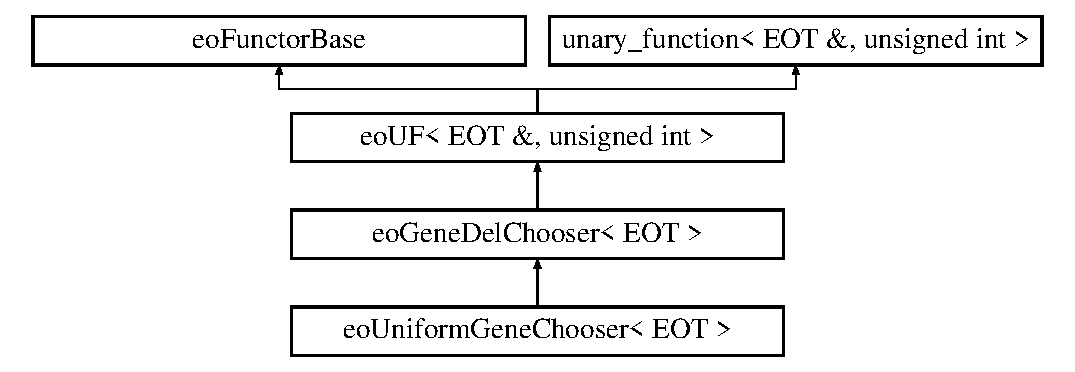
\includegraphics[height=4cm]{classeo_uniform_gene_chooser}
\end{center}
\end{figure}
\subsection*{Public Member Functions}
\begin{CompactItemize}
\item 
unsigned {\bf operator()} ({\bf EOT} \&\_\-eo)\label{classeo_uniform_gene_chooser_a1}

\begin{CompactList}\small\item\em The pure virtual function that needs to be implemented by the subclass. \item\end{CompactList}\item 
virtual std::string {\bf class\-Name} () const \label{classeo_uniform_gene_chooser_a2}

\end{CompactItemize}


\subsection{Detailed Description}
\subsubsection*{template$<$class EOT$>$ class eo\-Uniform\-Gene\-Chooser$<$ EOT $>$}

Uniform choice of gene to delete. 



Definition at line 94 of file eo\-Variable\-Length\-Mutation.h.

The documentation for this class was generated from the following file:\begin{CompactItemize}
\item 
eo\-Variable\-Length\-Mutation.h\end{CompactItemize}
